%%%%%%%%%%%%%%%%%%%%%%%%%%%%%%%%%%%%%%%%%
%
%%%%%%%%%%%%%%%%%%%%%%%%%%%%%%%%%%%%%%%%%

%----------------------------------------------------------------------------------------
%	PACKAGES AND OTHER DOCUMENT CONFIGURATIONS
%----------------------------------------------------------------------------------------


\documentclass[
11pt, % Main document font size
a4paper % Paper type, use 'letterpaper' for US Letter paper
%oneside, % One page layout (no page indentation)
%twoside, % Two page layout (page indentation for binding and different headers)
%headinclude,footinclude % Extra spacing for the header and footer
%BCOR5mm, % Binding correction
]{article}% ctexart
\usepackage{amsmath}
\usepackage{amsthm}
\newtheorem{Def}{Definition}
\newtheorem{Asp}{Assumption}
\usepackage{amsfonts}
\usepackage{amssymb}

\usepackage{chngcntr}
\theoremstyle{plain}

\let\origtheassumption\theassumption

\usepackage{verbatim}
\usepackage{bm}


%
 
\usepackage{graphicx} % support the \includegraphics command and options


%----------------------------------------------------------------------------------------
%	TITLE AND AUTHOR(S)
%----------------------------------------------------------------------------------------

\title{\normalfont{\huge Short Report on FFT in Hefei and Beijing Data}} % The article title%\spacedallcaps

\author{Yuzhe Zhang} % The article author(s) - author affiliations need to be specified in the AUTHOR AFFILIATIONS block
%\date{} % An optional date to appear under the author(s)

%----------------------------------------------------------------------------------------

\begin{document}
%----------------------------------------------------------------------------------------
%	AUTHOR AFFILIATIONS
%----------------------------------------------------------------------------------------
%\let\thefootnote\relax\footnotetext{\textsuperscript{*} \textit{Undergraduate Student,
% Department of Modern Physics, University of Science and Technology of China(USTC), Hefei, China}}
%----------------------------------------------------------------------------------------
\maketitle % Print the title/author/date block
%----------------------------------------------------------------------------------------
%	HEADERS
%----------------------------------------------------------------------------------------

%\newpage % Start the article content on the second page, remove this if you have a longer abstract that goes onto the second page

%----------------------------------------------------------------------------------------
%	TABLE OF CONTENTS & LISTS OF FIGURES AND TABLES
%----------------------------------------------------------------------------------------
\newpage

%\setcounter{tocdepth}{2} % Set the depth of the table of contents to show sections and subsections only

%\tableofcontents{} % Print the table of contents

%\listoffigures{} % Print the list of figures

%\listoftables{} % Print the list of tables

\section{Introduction}
I took Hefei and Beijing data on Jan.24, 2019, and apply FFT to it without other pretreatment. \\
Before we go into analysis, we have to be aware of the difficulty in data from stations. It did take some time to pick up a time when more than one stations are operating normally, which means there are data uploaded, and the data's sanity check is normal. I downloaded the data in January 2019 from the server. As far as I've checked, it's really tough to find a time when more than 4 stations are operating normally. I hope it's not like this in other period. 
\section{Result, Comparison and Analysis}
\subsection{FFT results of \textbf{Hefei} data from 13:09 to 19:22}
First, FFT results of \textbf{Hefei} data from 13:09 to 19:22 are presented below. In short, I found two suspicious spikes around 50 Hz and 253 Hz, besides 1/f noise around 0 Hz. As to 50 Hz, since the frequence of alternating current in China is 50 Hz, I am afraid that 50 Hz spike should be neglected. 
\newpage
\begin{figure}[ht]
	\centering
	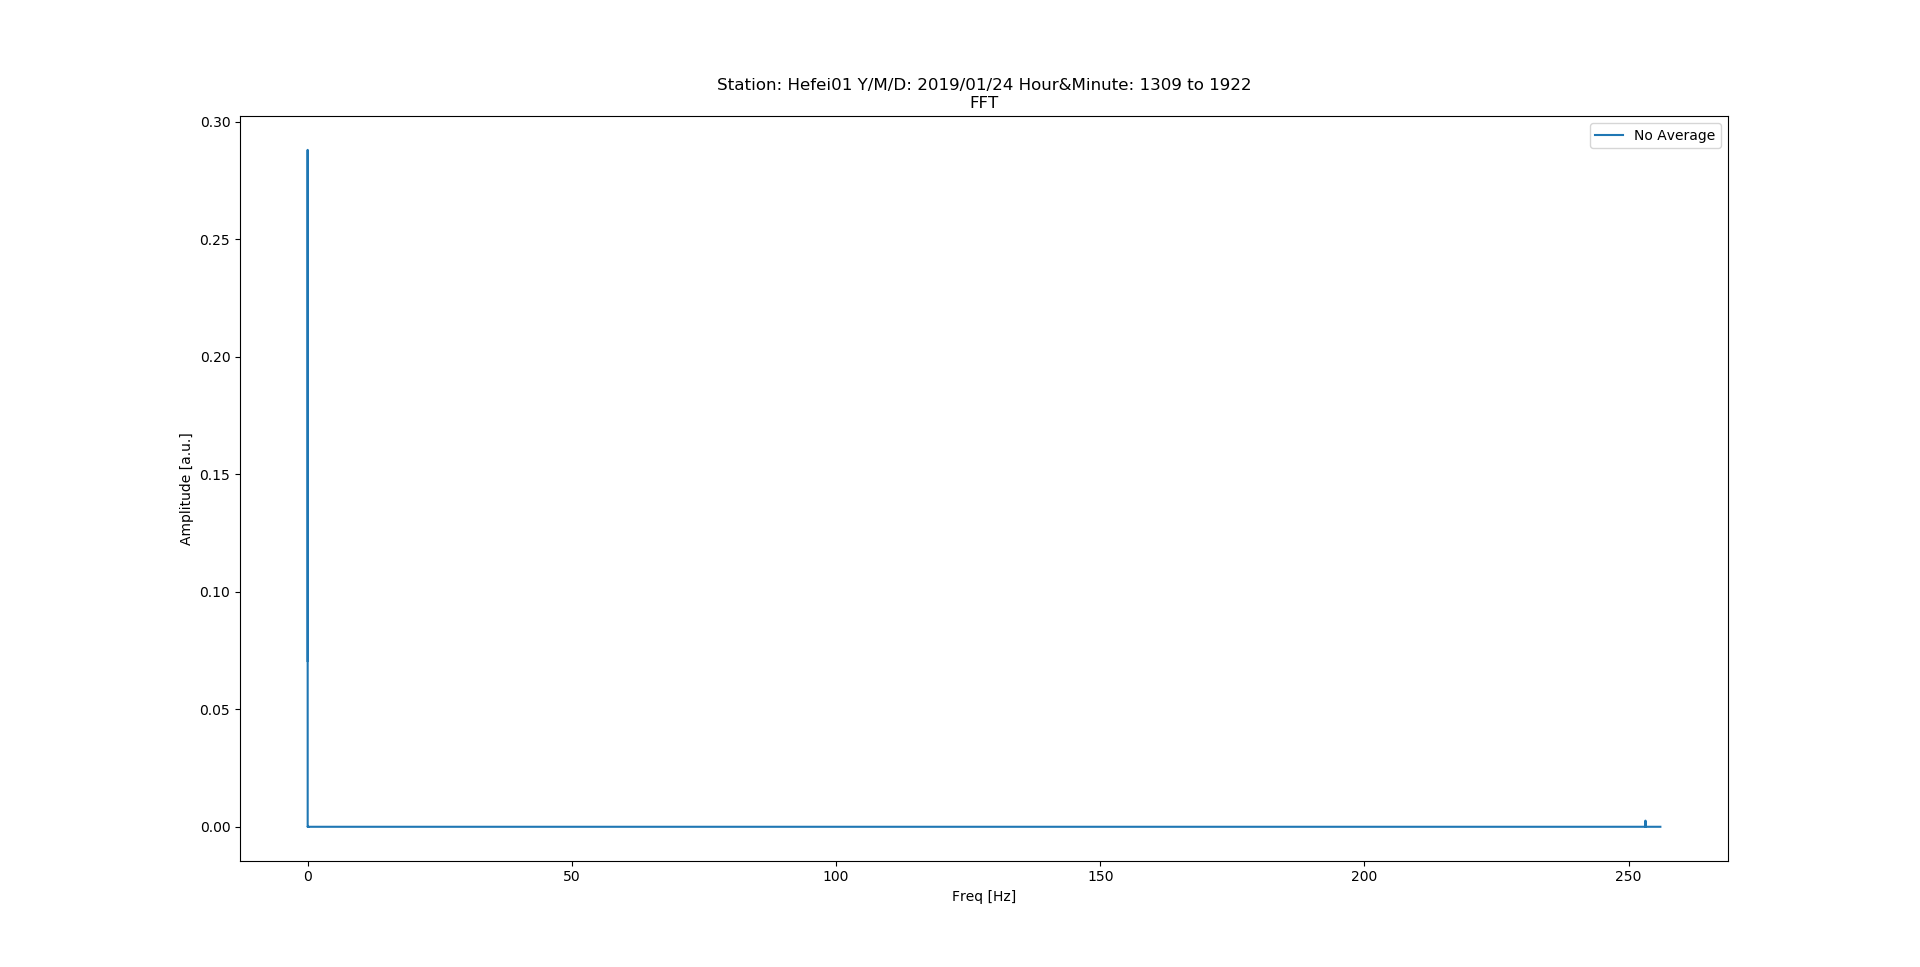
\includegraphics[width=\textwidth]{Figure_2.png}
	\caption{FFT result of Hefei data from 13:09 to 19:22}
	\label{fig:hefei2}
\end{figure}
\begin{figure}[ht]
	\centering
	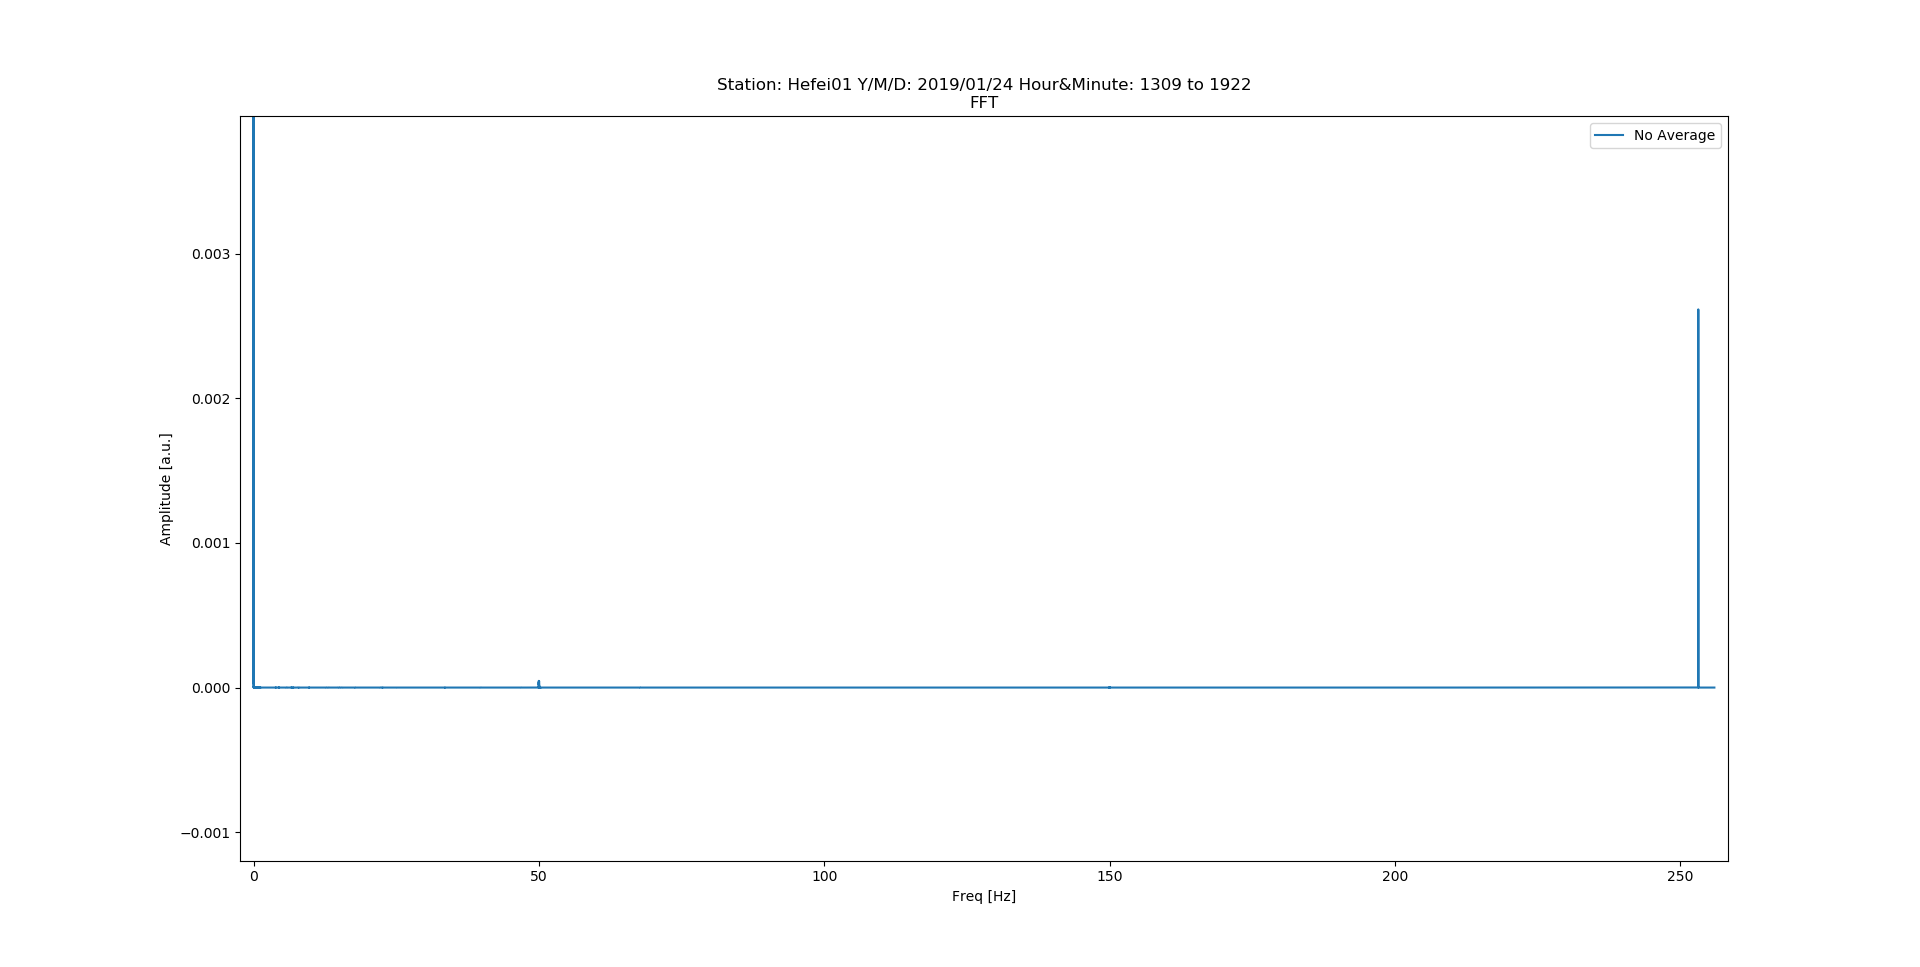
\includegraphics[width=\textwidth]{Figure_2_1.png}
	\caption{Zoomin in FFT result of Hefei data from 13:09 to 19:22. We can find \textbf{two spikes around 50 Hz and 253 Hz}}
	\label{fig:hefei2_1}
\end{figure}
\begin{figure}[ht]
	\centering
	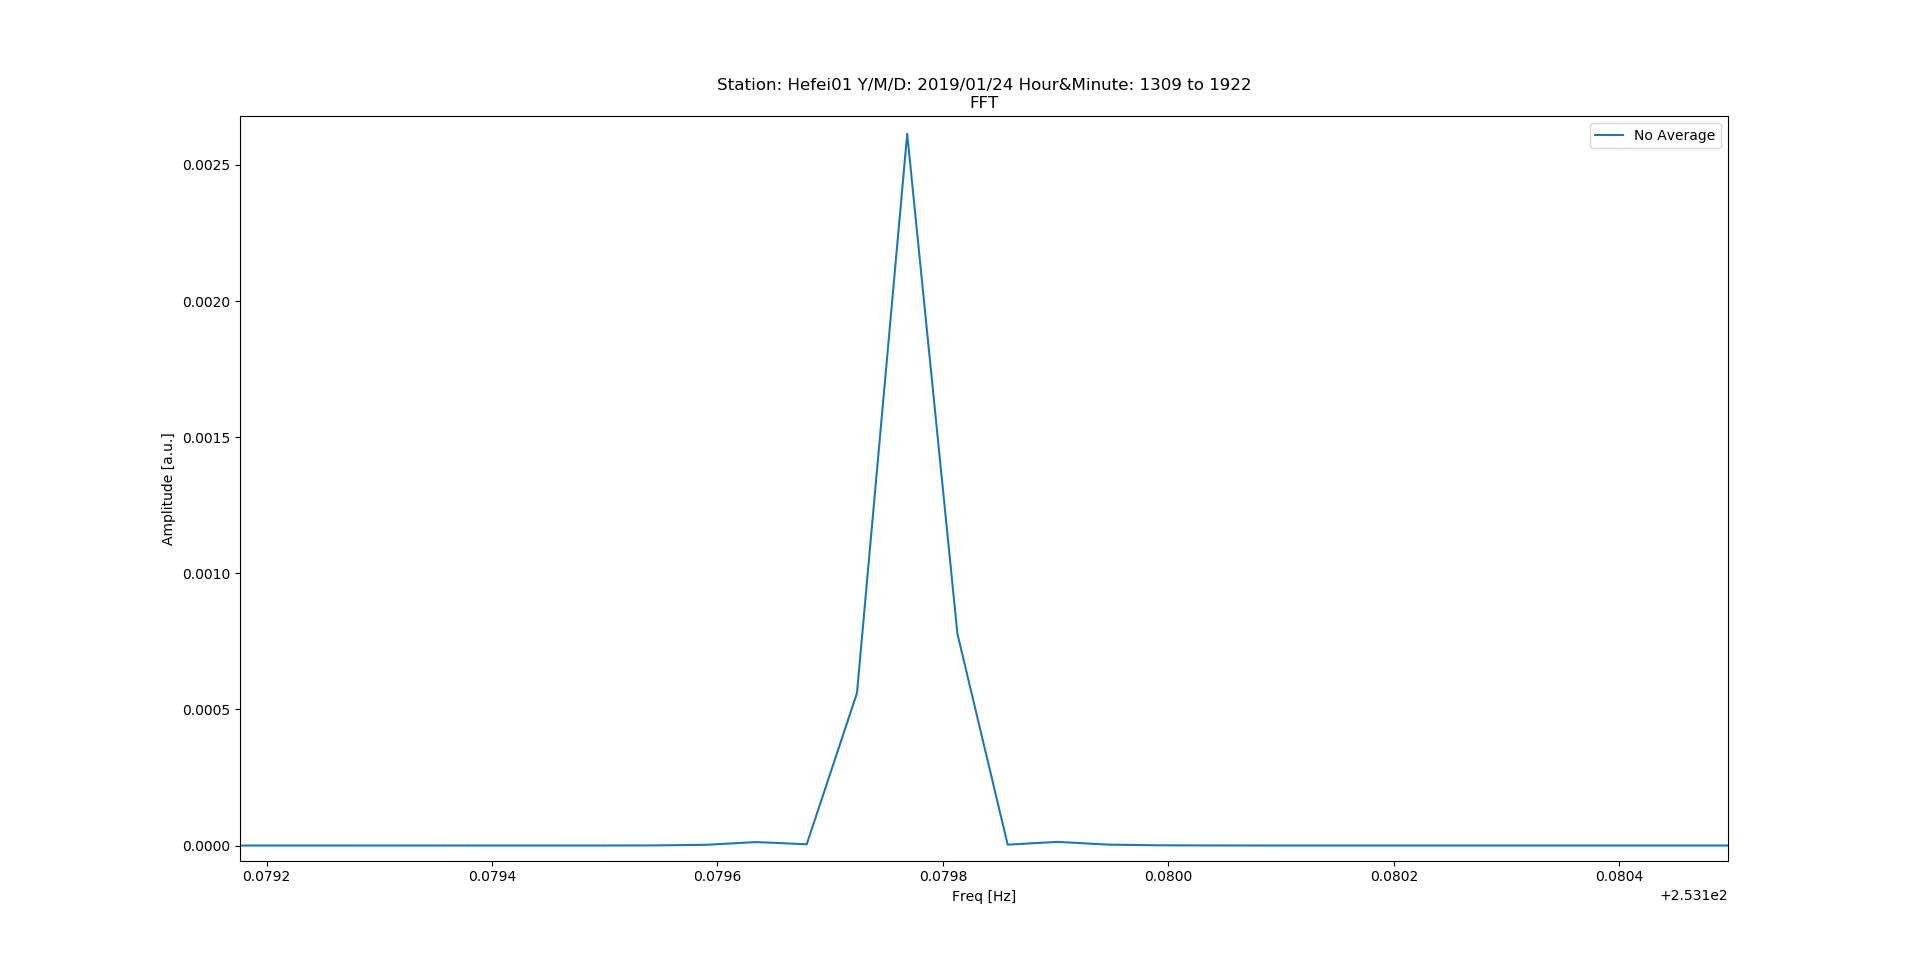
\includegraphics[width=\textwidth]{Figure_2_5.png}
	\caption{Zoomin in \textbf{Lorentz-like} Spike around \textbf{253 Hz} of FFT result of Hefei data from 13:09 to 19:22}
	\label{fig:hefei2_5}
\end{figure}
\newpage
\begin{figure}[h]
	\centering
	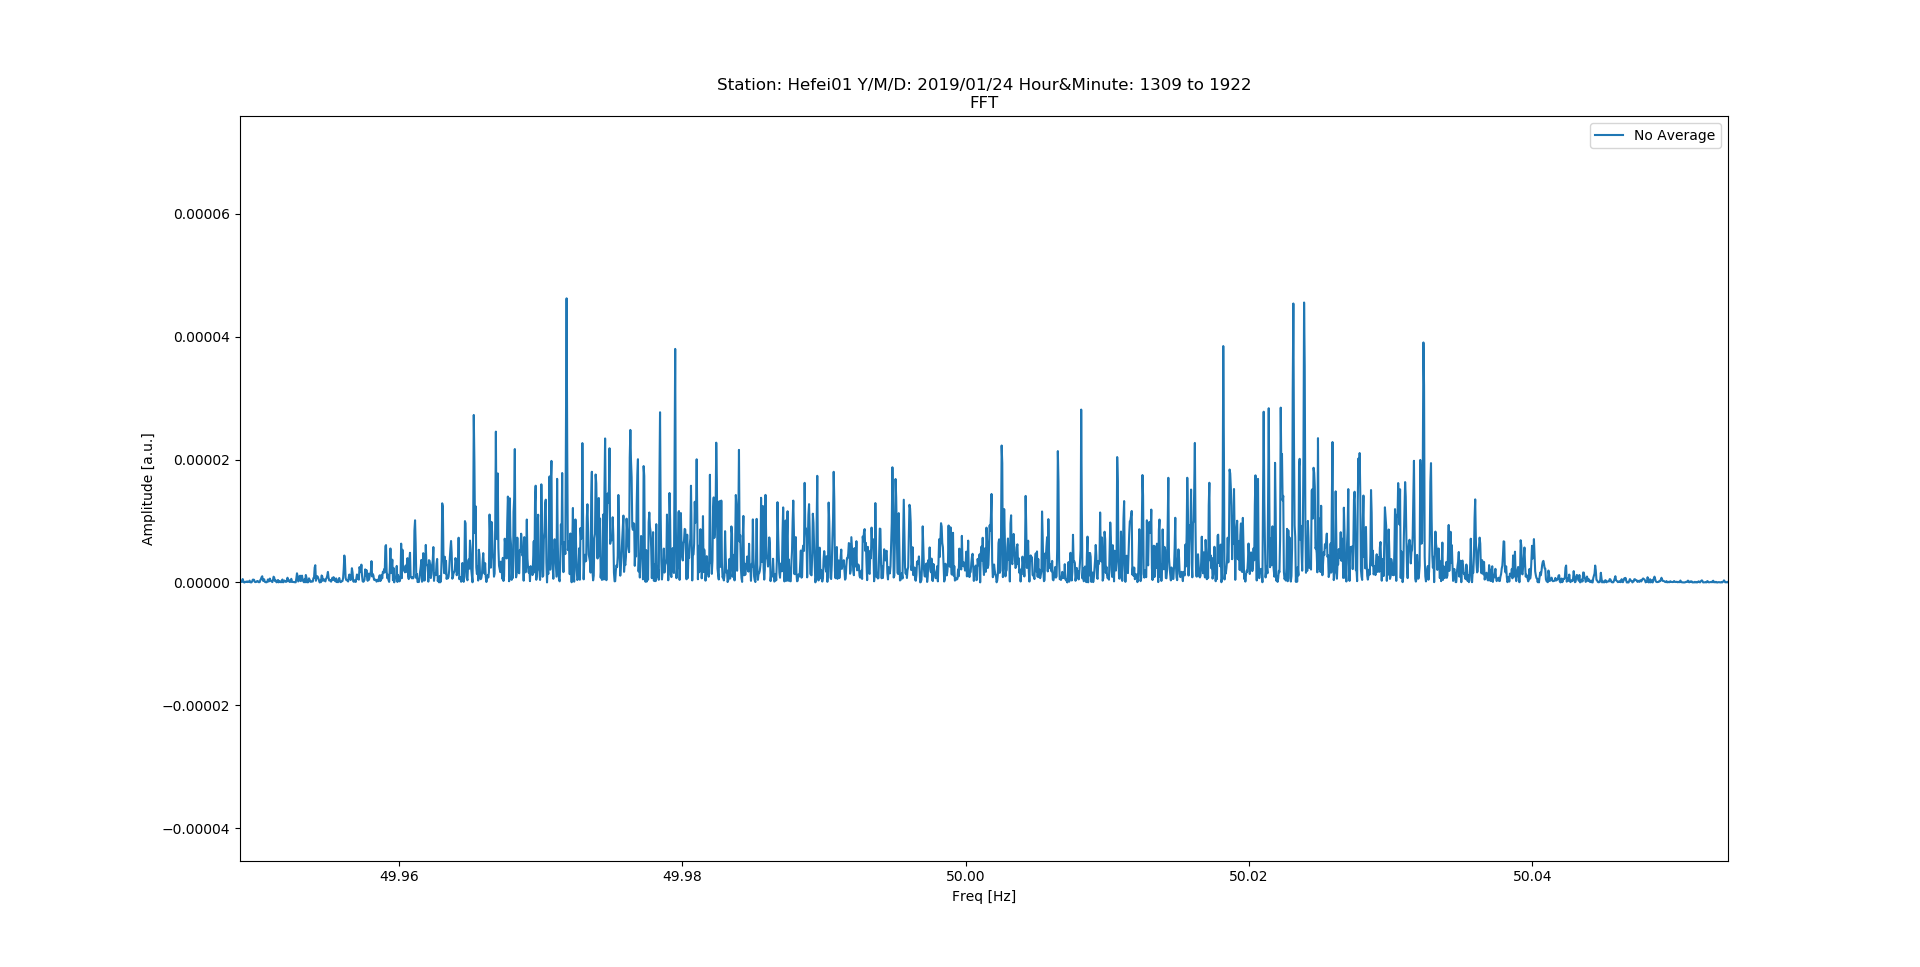
\includegraphics[width=\textwidth]{Figure_2_3.png}
	\caption{Zoomin in Spikes around \textbf{50 Hz} of FFT result of Hefei data from 13:09 to 19:22}
	\label{fig:hefei2_3}
\end{figure}
\newpage
\subsection{FFT results of \textbf{Beijing} data from 13:15 to 17:45}
Secondly, FFT results of \textbf{Beijing} data from 13:15 to 17:45 are presented below. In short, I found more suspicious spikes than in Hefei data. Among them, 50 Hz spike is tremendous. What we care about is whether the results from two stations have something in common. \\
I believe that 50 Hz spikes in Hefei and Beijing are both caused by China AC. The question is, are there spikes around 253 Hz like in Hefei? The answer is yes, but not apparent. \\
\newpage
\begin{figure}[ht]
	\centering
	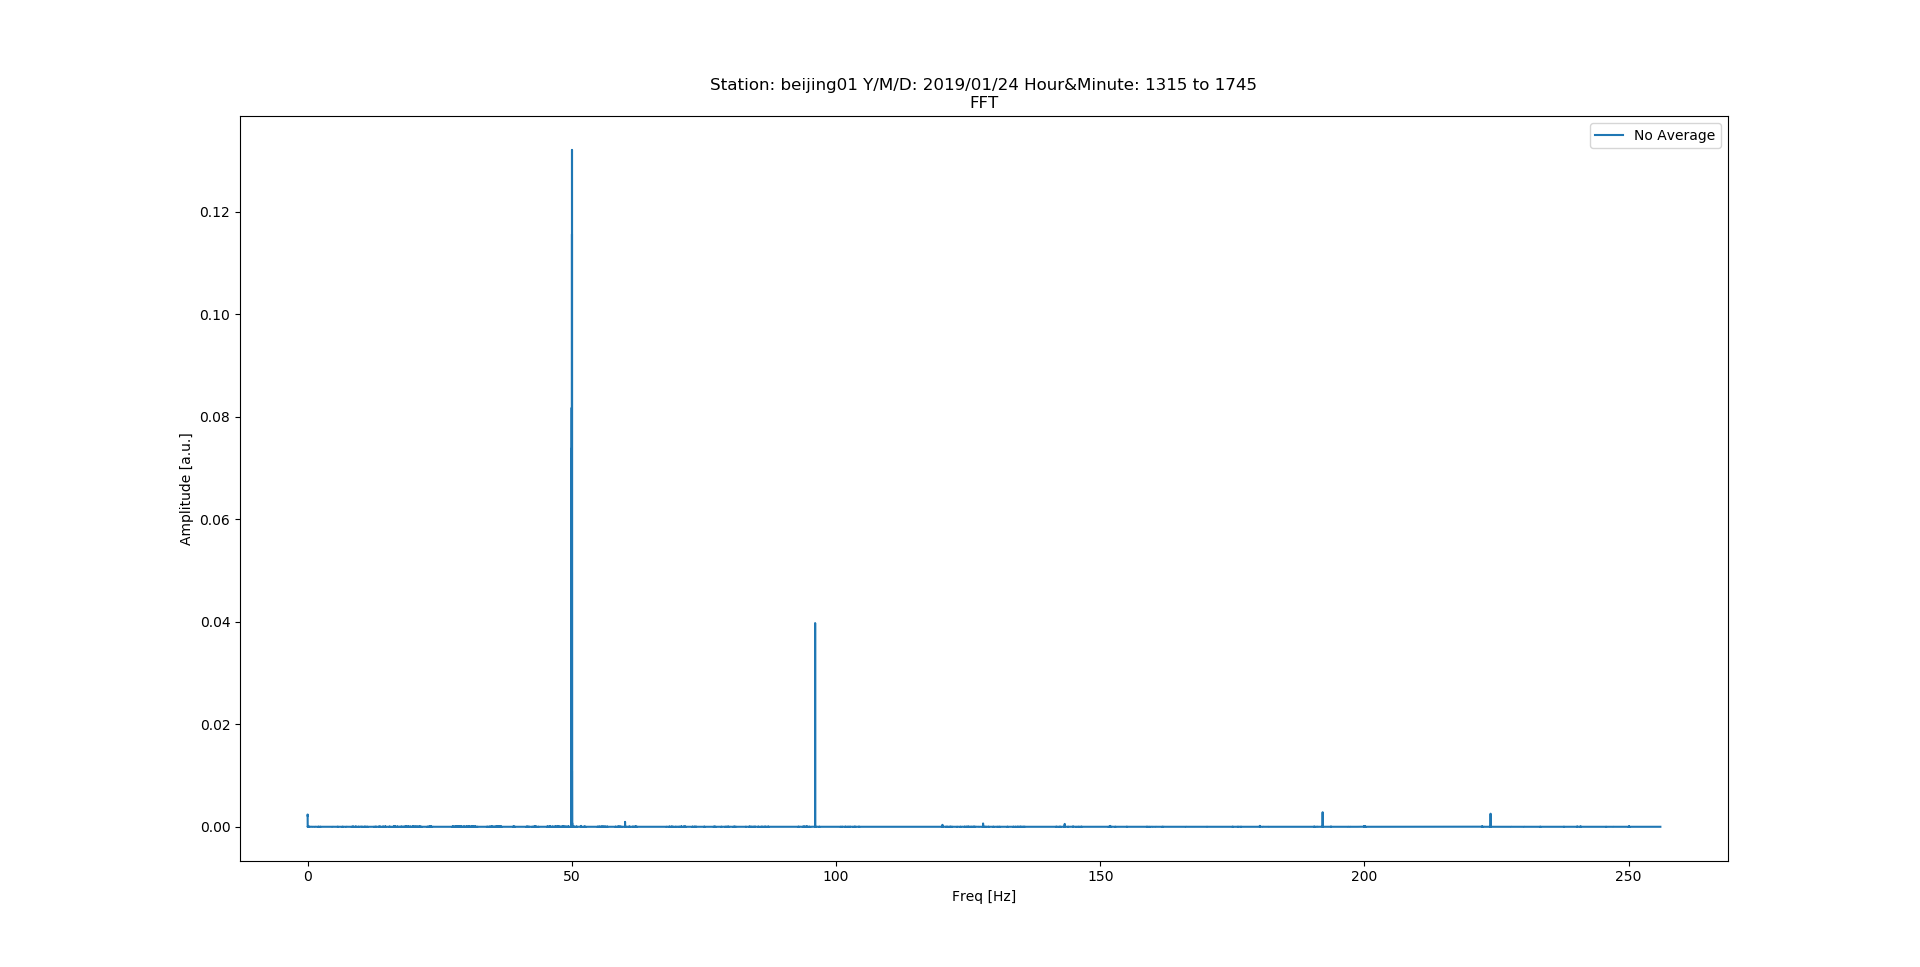
\includegraphics[width=\textwidth]{beijing2.png}
	\caption{FFT result of Beijing data from 13:15 to 17:45}
	\label{fig:beijing2}
\end{figure}
\begin{figure}[ht]
	\centering
	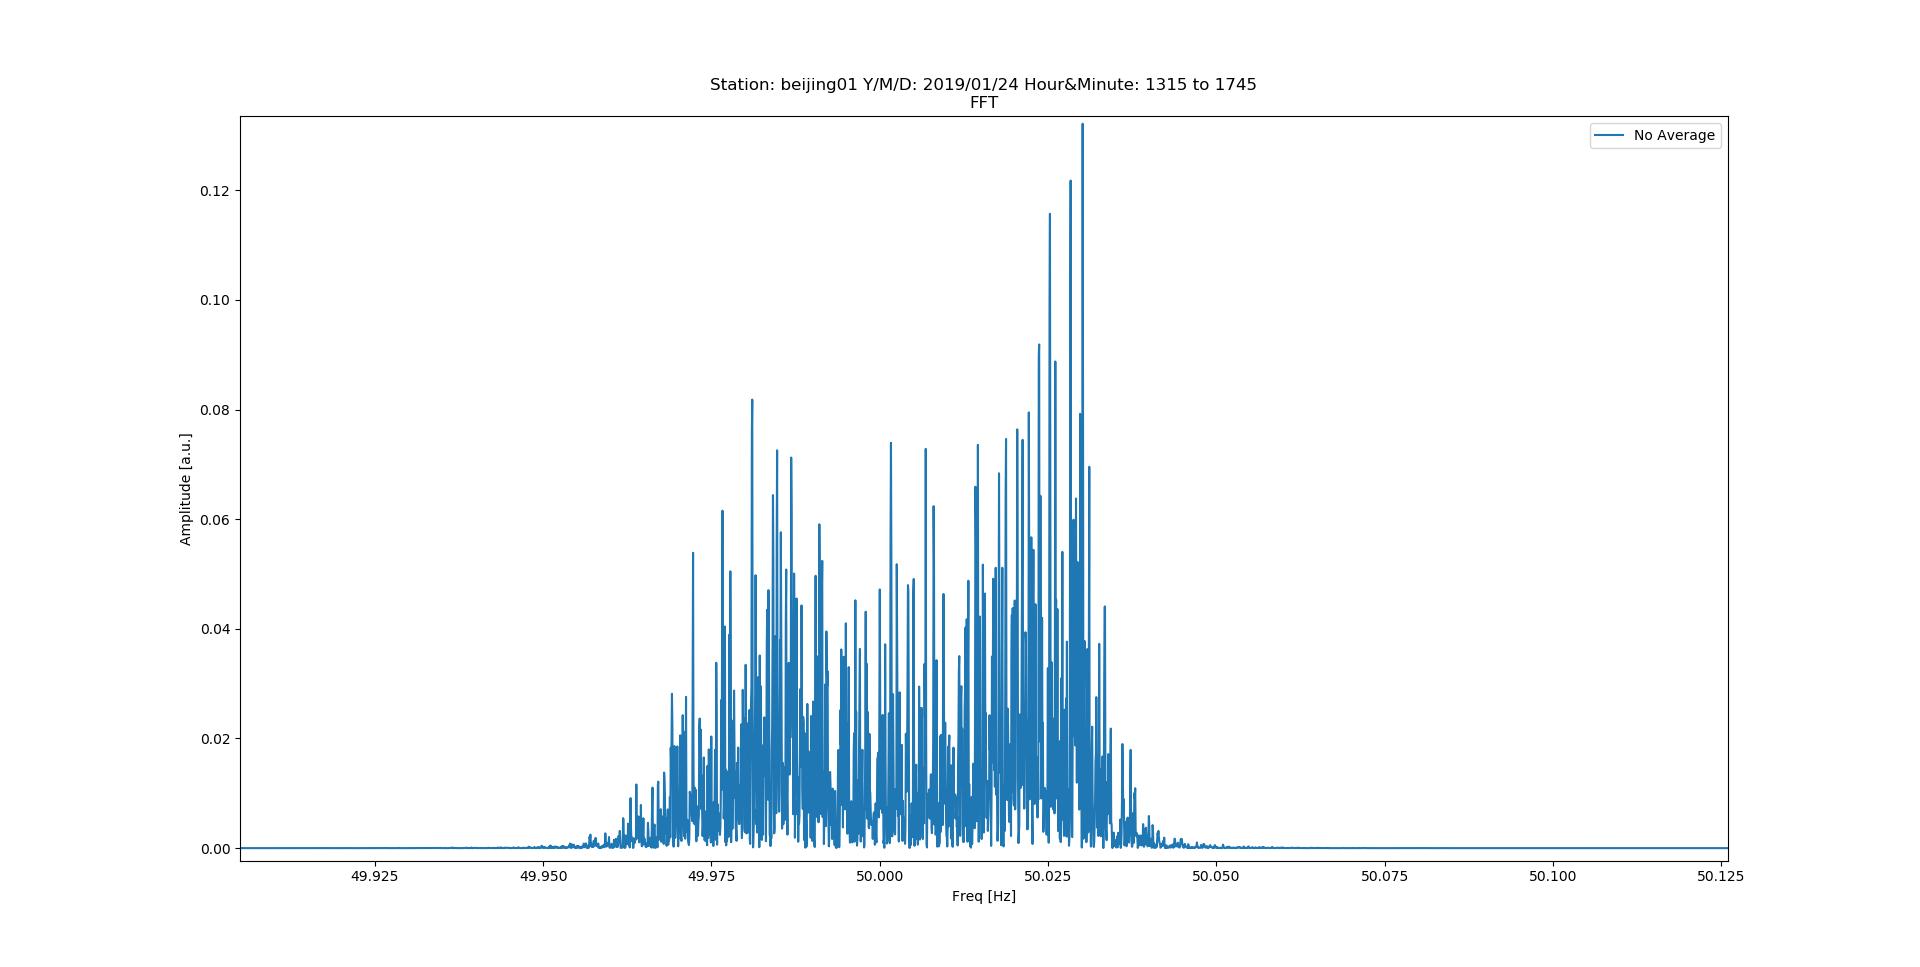
\includegraphics[width=\textwidth]{beijing2_0.png}
	\caption{Zoomin in \textbf{Spikes around 50 Hz} of FFT result of Beijing data from 13:15 to 17:45}
	\label{fig:beijing2_0}
\end{figure}
\newpage
\begin{figure}[ht]
	\centering
	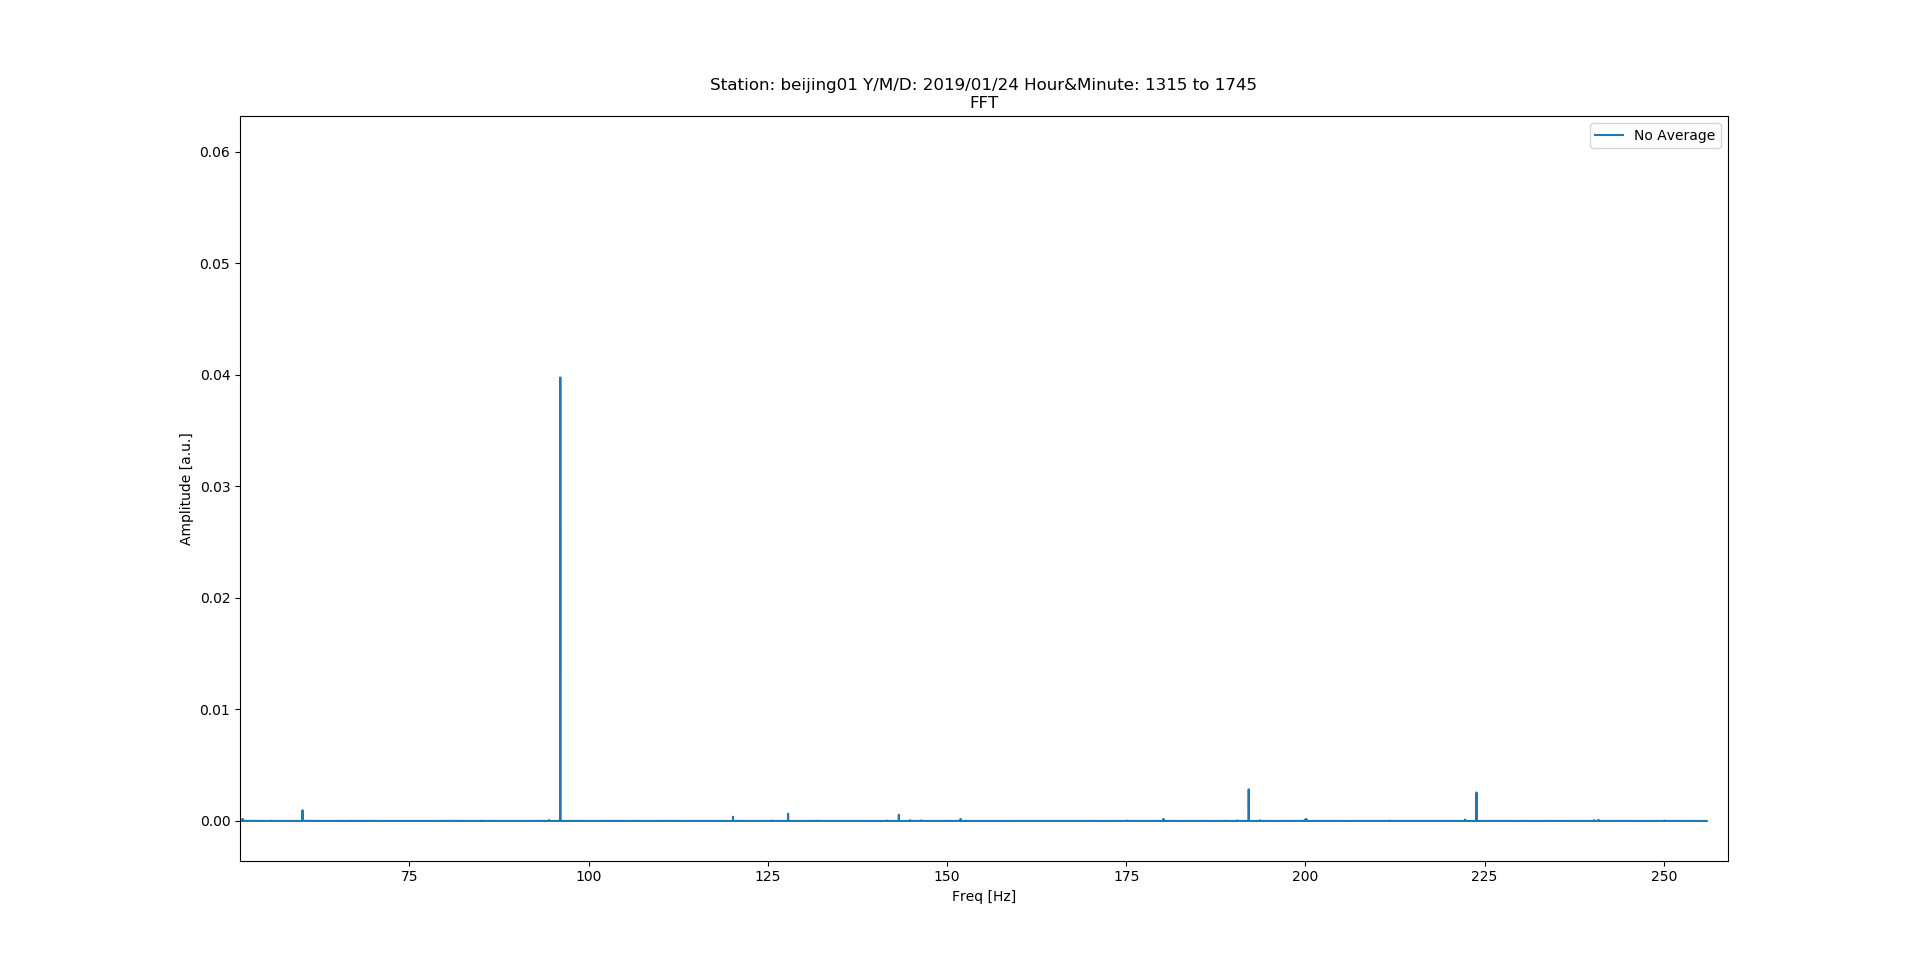
\includegraphics[width=\textwidth]{beijing2_2.png}
	\caption{Zoomin \textbf{above 50 Hz} of FFT result of Beijing data from 13:15 to 17:45. We can \textbf{hardly} see spikes around 253 Hz}
	\label{fig:beijing2_2}
\end{figure}
\newpage
\begin{figure}[htb]
	\centering
	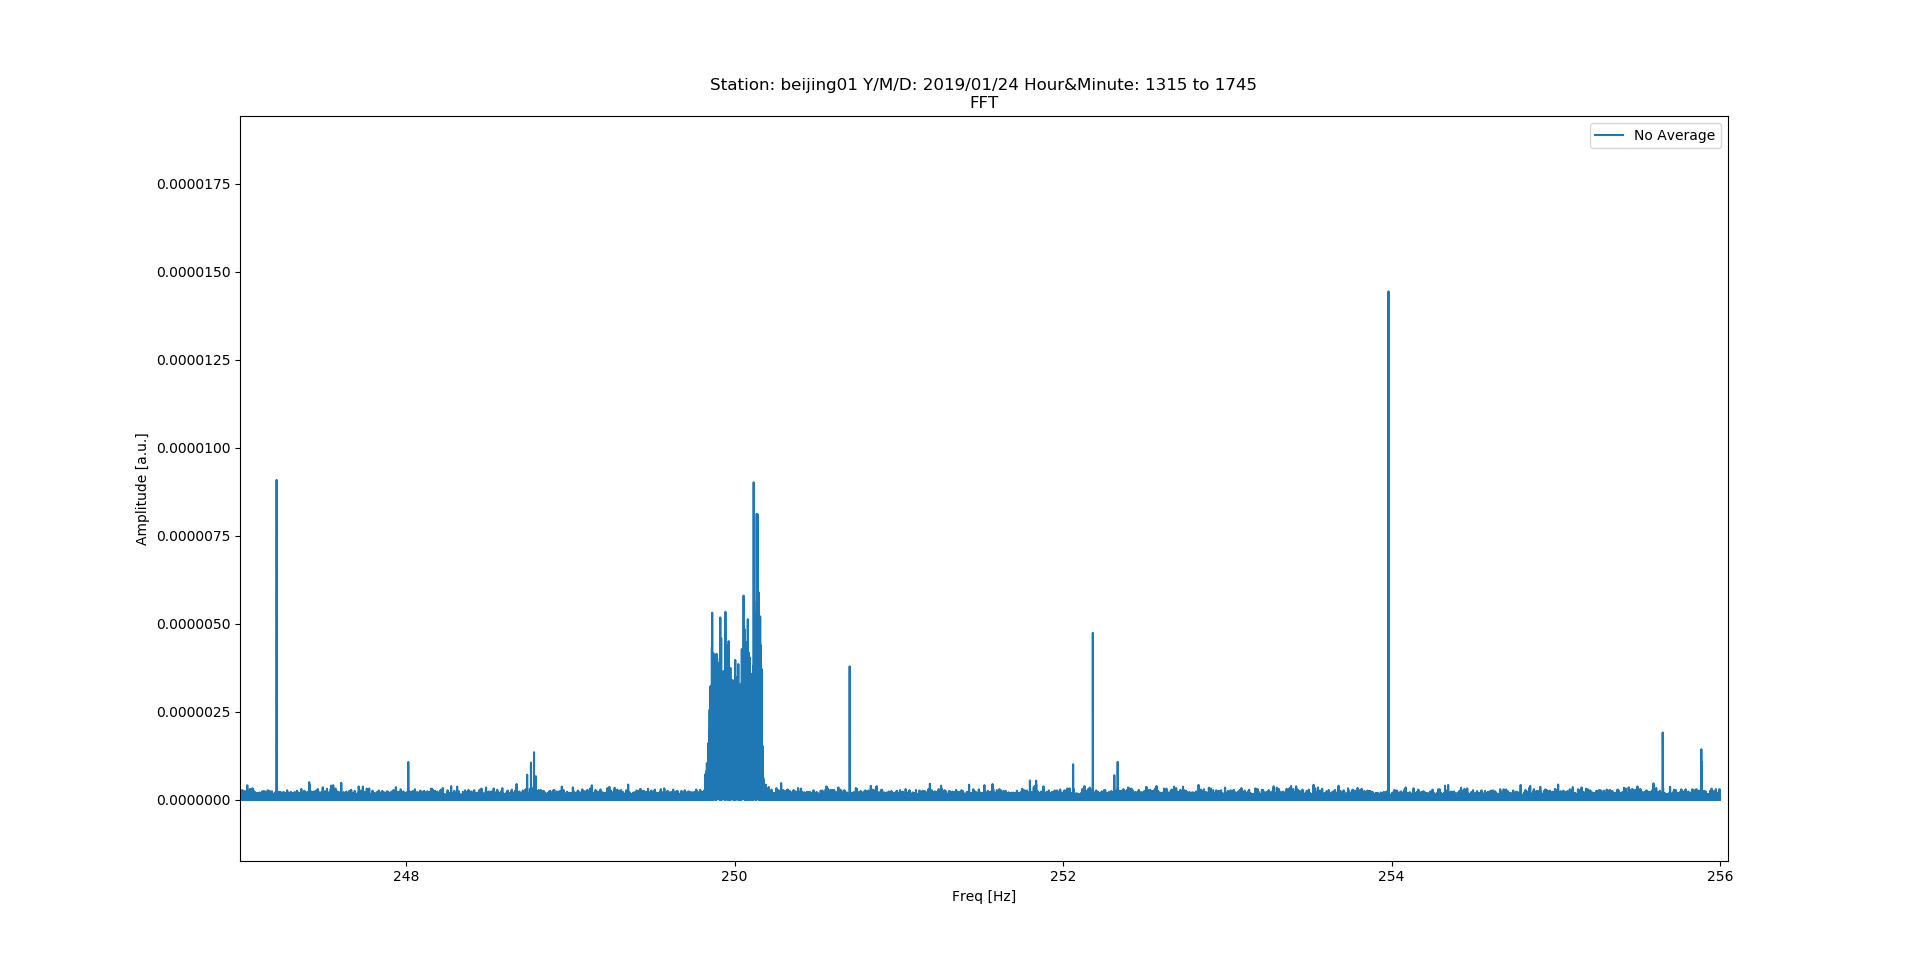
\includegraphics[width=\textwidth]{beijing2_1.png}
	\caption{Zoomin around \textbf{250 Hz} of FFT result of Beijing data from 13:15 to 17:45. We can \textbf{hardly} find 253 Hz spike like in Hefei. But we do see spikes near 253 Hz}
	\label{fig:beijing2_1}
\end{figure}
\newpage
\section{Conclusion}
%\newpage
After comparison in FFT result from two stations, we cannot conclude if we discovered anything due to the differences. Of course there would not be exactly same spikes in two stations. The question left to us is how to define coherence between stations when we do cross check, which indicates something more than noise in a single station. \\

%----------------------------------------------------------------------------------------
\end{document}